
\chapter{INTRODUÇÃO}
\label{chap:introducao}

% INTRODUÇÃO-------------------------------------------------------------------

O e-commerce, que em português significa comércio eletrônico, é uma modalidade de comércio que realiza suas transações financeiras por meio de dispositivos e plataformas eletrônicas, como computadores e celulares. Um exemplo deste tipo de comércio é comprar ou vender produtos em lojas virtuais. 
No início, o e-commerce era utilizado basicamente para vender bens tangíveis com valores modestos, como: livros e CDs. Hoje, ele é utilizado para comercializar desde produtos que custam milhões, como: iates, carros de luxo e mansões, até produtos que há pouco tempo eram inimagináveis pela sua incompatibilidade com este tipo de comércio, como roupas, perfumes e alimentos. \cite{ecomm} %%ver data da postagem no site??

%%% Verifica a inserção desta parte no trabalho. 
%Segundo \cite{gestcont}, o e-commerce permite que os consumidores transacionem bens e serviços eletronicamente sem barreiras de tempo ou distância.

Sabe-se que atualmente está sendo mais frequente o uso de lojas virtuais para realizar compras sem ser necessário fazer a locomoção para poder adquirir o produto desejado. Pensando no crescimento do comércio eletrônico, foi proposto no presente trabalho o desenvolvimento de um e-commerce voltado para moda, roupas e acessórios. 

Este trabalho será desenvolvido utilizando a linguagem de programação PHP juntamente com CSS, HTML, Javascript e  utilizando banco de dados MySql.
No decorrer das aulas foi realizada a documentação do trabalho contendo os diagramas UML, sendo compreendido e relatado nos seguintes capítulos descritos abaixo.

%Seção Tecnologias
Na seção primária \ref{chap:tec} é relatado as linguagens que serão utilizadas no decorrer do desenvolvimento do sistema.

%Seção Definição dos atores, Diagramas de Casos de Usos e Descrição dos Casos de Uso
Na seção secundária \ref{sec:anareq}, a seção terciária \ref{sec:defatores}, \ref{sec:casuso} e \ref{sec:conuso}, está descrito os atores, diagramas de casos de uso e suas descrições.

%Seção do Diagrama de Classe
A seção secundária \ref{sec:modcon} e a seção terciária \ref{sec:diacla} trata-se da modelagem conceitual contendo o diagrama de classes juntamente com a identificação entre essas classes.

%Seção do Diagrama de Sequência
Na seção secundária \ref{sec:modcom} e seção terciária \ref{sec:conseq} e \ref{sec:diaati} foi construído os diagramas de sequência e diagrama de atividades.


\chapter{ESCOPO}
\label{chap:escopo}

O seguinte projeto possui página principal que irá conter informações referentes à história do site, menu para pesquisa de itens, uma sacola para adicionar os produtos, como roupas e acessórios escolhidos durante a compra.

\chapter{TECNOLOGIAS UTILIZADAS}
\label{chap:tec}

O trabalho foi planejado para ser desenvolvido com as seguintes linguagens, sendo tratado de uma estrutura própria, de início não será utilizado nenhum framework, considerando que o projeto ainda não foi iniciado, está possível de ser alterado qualquer uma das linguagens citadas abaixo.

\section{HTML}
 \textit{HTML} é uma das linguagens que utilizamos para desenvolver websites. O acrônimo HTML vem do inglês e significa Hypertext Markup Language ou em português Linguagem de Marcação de Hipertexto. O HTML é a liguagem base da internet. Foi criada para ser de fácil entendimento por seres humanos e também por máquinas, como por exemplo o Google ou outros sistemas que percorrem a internet capturando informação.\cite{html}

\section{CSS}
O Cascading Style Sheets  (\textit{CSS}) é uma "folha de estilo" composta por “camadas” e utilizada para definir a apresentação (aparência) em páginas da internet que adotam para o seu desenvolvimento linguagens de marcação (como  \textit{XML, HTML e XHTML}). O CSS define como serão exibidos os elementos contidos no código de uma página da internet e sua maior vantagem é efetuar a separação entre o formato e o conteúdo de um documento. \cite{css1}.

Quando falamos de acessibilidade, performance e manutenção, tem-se como princípio fazer separação do conteúdo, da interatividade e da apresentação de um site ou aplicação web. O CSS desempenha um grande papel na camada da apresentação.
A forma certa de publicar um documento web é seguindo uma estrutura semântica. O CSS traz toda a informação do layout, isto é, cores, posicionamento, fontes, tamanhos e imagens de fundo, enquanto o HTML deve fornecer uma “arquitetura” para o conteúdo. \cite{css2}

\section{PHP}

A sigla  \textit{PHP} vem do inglês Personal Home Page que traduzido para o português significa página pessoal principal. Normalmente as páginas web são feitas com código de hipertexto (um código que permite a ligação de palavras a outros sites da internet ou a outros da mesma página). No caso da PHP este código pode ser encontrado no código HTML ou hipertexto.

O PHP é um código usado por ser fácil de aprender e ainda por cima grátis. Muita gente aprende porque é muito solicitado na criação de páginas web corporativas e pessoais, no entanto, é necessário certo conhecimento básico de informática, especialmente de código HTML. Ele pode ser incorporado obrigatoriamente aos servidores de página web e produzir animações, efeitos variados de cores, movimentos de certos elementos, etc. Seus efeitos visuais podem ser desde muito simples até animações bem complexas, da mesma forma das que aparecem às vezes na página principal do Google. \cite{php}

\section{MySQL}

O  \textit{MySQL} é um sistema gerenciador de banco de dados relacional de código aberto usado na maioria das aplicações gratuitas para gerir suas bases de dados. O serviço utiliza a linguagem  \textit{SQL}x' (Structure Query Language – Linguagem de Consulta Estruturada), que é a linguagem mais popular para inserir, acessar e gerenciar o conteúdo armazenado num banco de dados.
a criação de aplicações web abertas e gratuitas, o conjunto de aplicações mais usado é o LAMP, um acrônimo para Linux, Apache, \textit{MySQL e Perl/PHP/Python}. Nesse conjunto de aplicações, inclui-se, respectivamente, um sistema operacional, um servidor web, um sistema gerenciador de banco de dados e uma linguagem de programação. Assim, o MySQL é um dos componentes centrais da maioria das aplicações públicas da Internet. \cite{mysql}

\section{Git}
\textit{GIT} é um dos vários Sistemas de Controle de Versão de arquivos, permite que você registre as mudanças feitas em um arquivo ou um conjunto de arquivos ao longo do tempo de forma que se possa recuperar versões específicas. Um Sistema de Controle de Versão \textit{(VCS)} também permite que você reverta arquivos para um estado anterior, compare mudanças feitas no decorrer do tempo, veja quem foi o último a modificar algo que pode estar causando problemas, ou quem introduziu um bug e quando, além de muitas outras alternativas. E tem mais, se você estiver usando um VCS não precisará se preocupar se o computador estragou ou se perdeu algum arquivo, pois com o sistema poderá facilmente reavê-los. \cite{git}

\section{Github}
\textit{Github} (palavra que seria traduzida como "agregador de gits") é o site mais conhecido de hospedagem de projetos git, ele serve para que você e sua equipe possam manter as versões do projeto em que trabalham em um lugar centralizado, na internet, acessível a quem pertence ao projeto. Além de hospedar projetos git, o github dá visibilidade da linha do tempo de diferentes versões do projeto, provê ferramentas de métricas (como quais usuários alteraram mais o projeto, quando alteraram, o que alteraram, etc), gerência de problemas relatados (\textit{tickets} ou \textit{issues}), dentre outras. \cite{github}

%%%%%%%%%%%%%%%%%%%%%%______________________________%%%%%%%%%%%%%%%%%%%%%%______________________________%%%%%%%%%%%%%%%%%%%%%%______________________________


\chapter{DIAGRAMA UML}
\label{chap:diauml}
A Unified Modeling Language ou Linguagem de Modelagem Unificada \textit{UML}, é uma linguagem visual utilizada para modelar softwares baseados no paradigma de orientação a objetos. A linguagem pode ser aplicada a todos os domínios de aplicação pois possui um propósito geral e se tornou, nos últimos anos, a linguagem padrão de modelagem adotada pelos engenheiros de software de todo o mundo. \cite{Guedes}

Segundo \cite{Alberto}, a UML apresenta as seguintes características principais:
É independente do domínio de aplicação, pode ser usado em projetos de diferentes características, tais como sistemas cliente/servidor tradicionais; sistemas baseados na Web; sistemas de informação geográficos; sistemas de tempo real); é independente do processo ou metodologia de desenvolvimento; é independente das ferramentas de modelagem; apresenta mecanismos potentes de extensão; agrega um conjunto muito significativo de diferentes diagramas/técnicas dispersos por diferentes linguagens, diagramas de casos de utilização, de classes, de objetos, de colaboração, de atividades, de estados, de componentes, e de instalação). 

\section{Análise de Requisitos}
\label{sec:anareq}
%%%%%%--------------------------------------------------------------------------------------------%%%%%%
\subsection{Definição dos Atores}
\label{sec:defatores}
Os atores são peças fundamentais para que o sistema tome forma, pois serão os responsáveis pelo funcionamento de todo e qualquer sistema, deste modo os atores relatados durante o desenvolvimento deste projeto trata-se do cliente, ou seja, pessoas, usuários que serão responsáveis por realizar as compras, realizar pesquisas entre os produtos, efetuar pagamentos, bem como o uso do 'ator' sistema, que este dá o embasamento para o usuário poder fazer a utilização do site.

\subsection{Casos de Uso}
\label{sec:casuso}
Diagrama de casos de uso é um diagrama muito importante de ser utilizado devido às vantagens que se pode ter, pensando na possibilidade de desenvolver um sistema voltado para um cliente. Esses diagramas são muito claros e visíveis para o usuário explicar o que ele realmente deseja que o sistema faça, e sendo mais claro para o analista de projeto fazer a análise das informações.

\begin{figure}[H]
    \centering
    \caption{Diagrama de Caso de Uso -  Realizar Compra}
    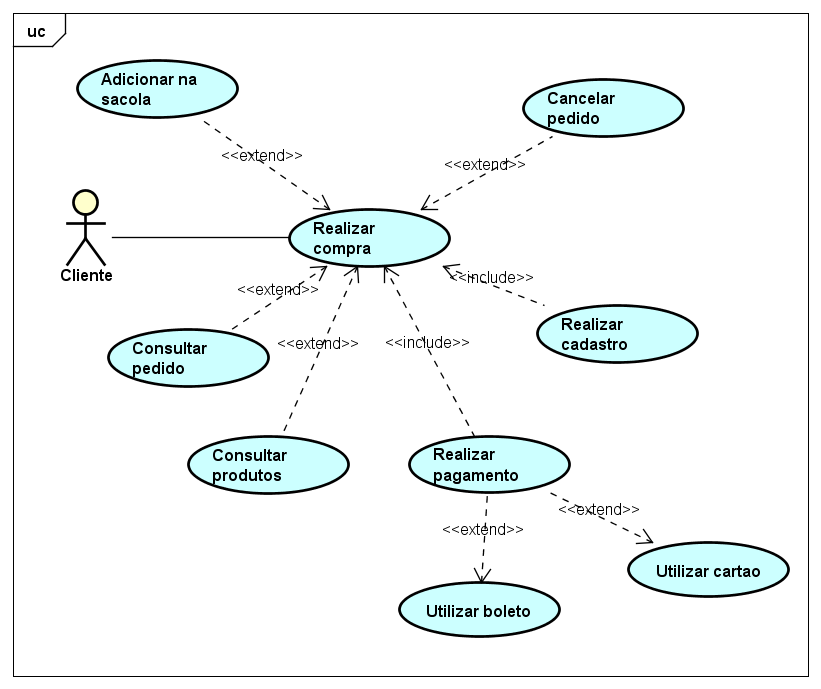
\includegraphics[width=1.0\textwidth]{./dados/figuras/4_1}
    \fonte{Autor}
    \label{fig:figura-1}
\end{figure}
No caso de uso realizar compra, Figura \ref{fig:figura-1}, o usuário precisa estar cadastrado no banco de dados e assim deve escolher a forma de pagamento onde se trata da utilização de boleto bancário ou cartão de crédito. Usuário precisa adicionar o produto na sacola para que a compra seja concluída, sendo assim ele pode realizar a consulta do pedido e se necessário, está apto a realizar o cancelamento do mesmo.
%%-------------------------------------------%%

\begin{figure}[H]
    \centering
    \caption{Diagrama de Caso de Uso - Realizar Cadastro}
    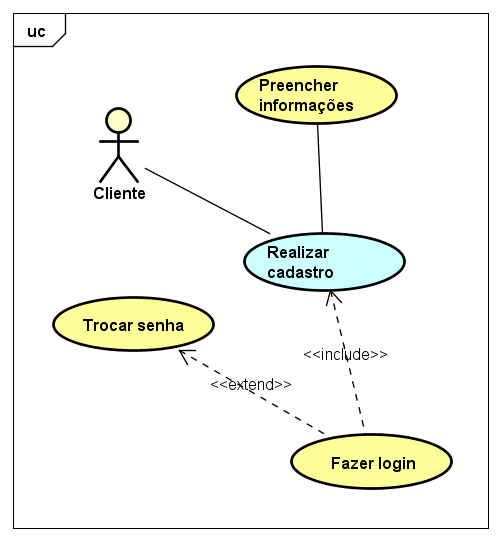
\includegraphics[width=0.5\textwidth]{./dados/figuras/4_2}
    \fonte{Autor}
    \label{fig:figura-2}
\end{figure}
Na Figura \ref{fig:figura-2} o usuário irá realizar o preenchimento dos dados pessoais para realizar o cadastro e também pode realizar a troca da senha, se necessário.

%%%%%%--------------------------------------------------------------------------------------------%%%%%%
\subsection{Descrição dos Casos de Uso}
\label{sec:conuso}

\begin{figure}[H]
    \centering
    \caption{Descrição do Caso de Uso -  Realizar Compra}
    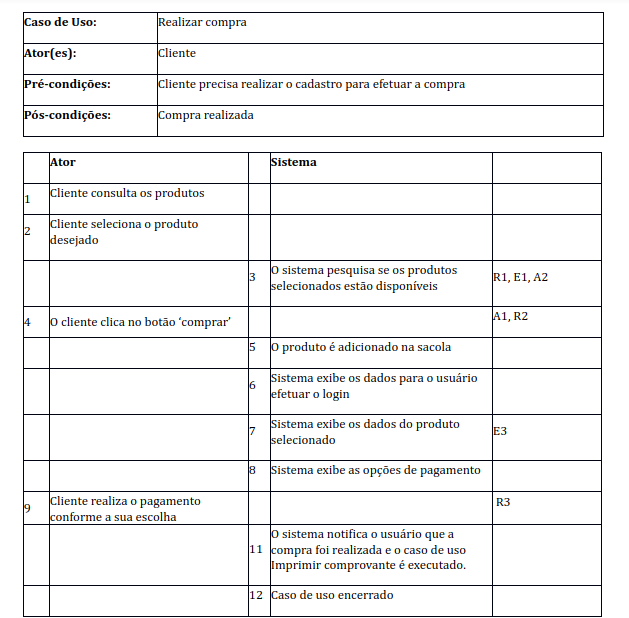
\includegraphics[width=1.0\textwidth]{./dados/figuras/Compra1}
    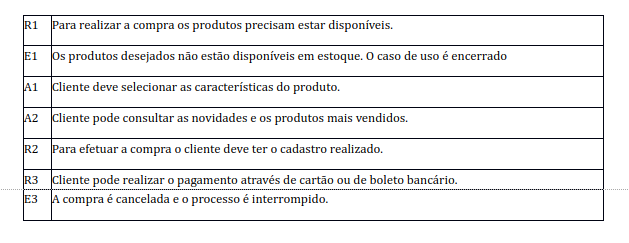
\includegraphics[width=1.0\textwidth]{./dados/figuras/1_2}
    \fonte{Autor}
    \label{fig:figura-3}
\end{figure}
\begin{figure}[H]  %!htb
    \centering
    \caption{Descrição do Caso de Uso -  Realizar Cadastro e Efetuar Login}
    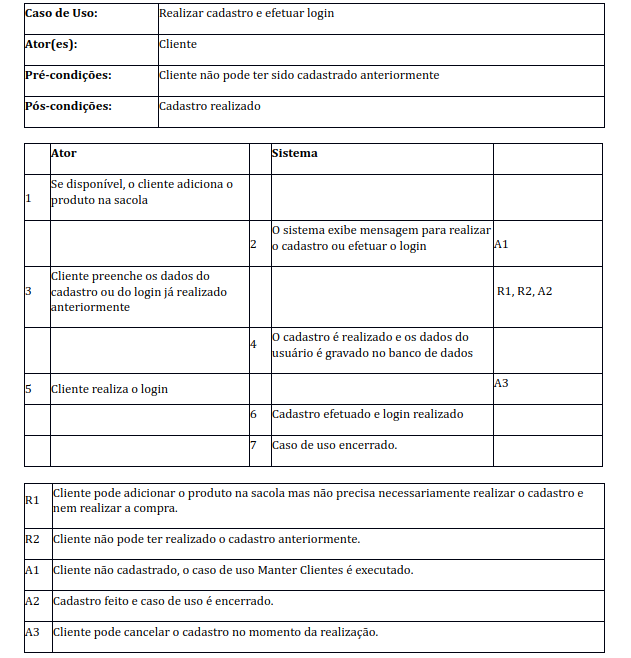
\includegraphics[width=1.0\textwidth]{./dados/figuras/2}
    \fonte{Autor}
    \label{fig:figura-4}
\end{figure}

A descrição dos casos de usos, conforme visto na Figura \ref{fig:figura-3} e \ref{fig:figura-4} são explicadas passo a passo na própria imagem, na qual possui o usuário como sendo um ator e o sistema para ajudar com o processo. Na descrição do caso de uso é explicado a lógica do funcionamento do site, ou seja, passo a passo de como o site irá se comportar considerando o processo de realizar cadastro e realizar compra. Possui algumas regras cruciais que precisam ser seguidas.  
%%%%%%--------------------------------------------------------------------------------------------%%%%%%

\section{Modelagem Conceitual}
\label{sec:modcon}

\subsection{Diagrama de Classes de Análise}
\label{sec:diacla}
O principal enfoque do diagrama de classes de análise está em permitir a visualização das classes que irão compor o sistema com seus respectivos atributos e métodos, bem como em demonstrar como as classes do sistema se relacionam, se complementam e transmitem informações entre si. Este diagrama apresenta uma visão estática de como as classes estão organizadas, preocupando-se em definir a estrutura lógica das mesmas. O diagrama de classes serve como base para a construção da maior parte dos demais diagramas da UML. \cite{class}
 
\begin{figure}[H]
    \centering
    \caption{Diagrama de Classe}
    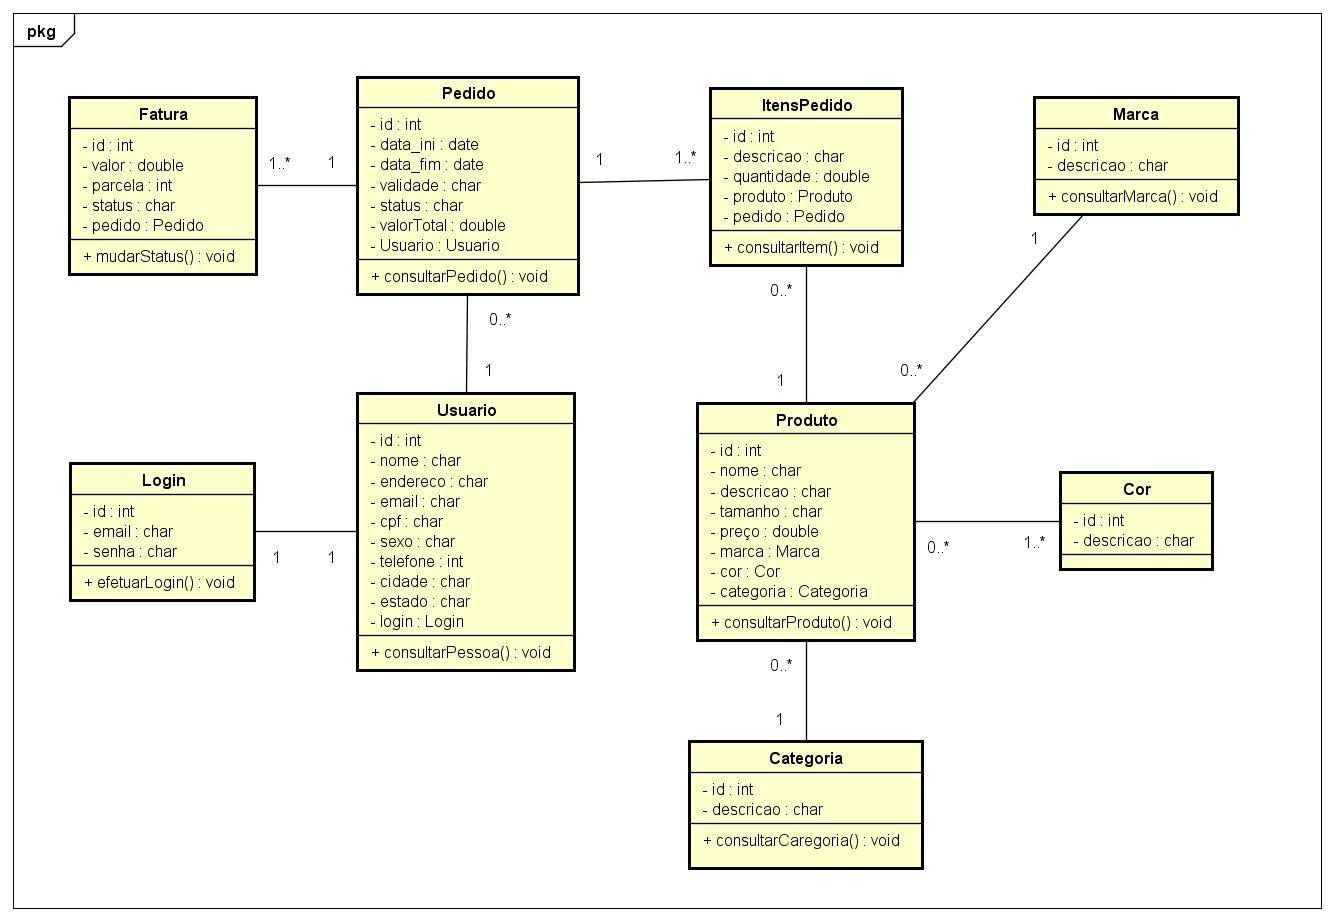
\includegraphics[width=1.0\textwidth]{./dados/figuras/5}
    \fonte{Autor}
    \label{fig:figura-5}
\end{figure}

A Figura \ref{fig:figura-5} mostra o diagrama de classes que representa todas as classes do projeto com suas respectivas associações e atributos.
%%%%%%%%%%%

%Adicionar descrição para os demais conceitos ainda não listados no trabalho

%%
\section{Modelagem comportamental}
\label{sec:modcom}

\subsection{Construção dos Diagramas de Sequência}
\label{sec:conseq}
O diagrama de sequência é uma ferramenta que deve ser utilizada sempre em  função dos casos de uso. Um diagrama de sequência captura o comportamento de  um único caso de uso, ou seja, mostra a interação entre os objetos ao longo  do tempo, apresentando os objetos que participam da interação e a sequência das mensagens trocadas. \cite{Atividade}

\begin{figure}[H]
    \centering
    \caption{Diagrama de Sequência - Fazer Login}
    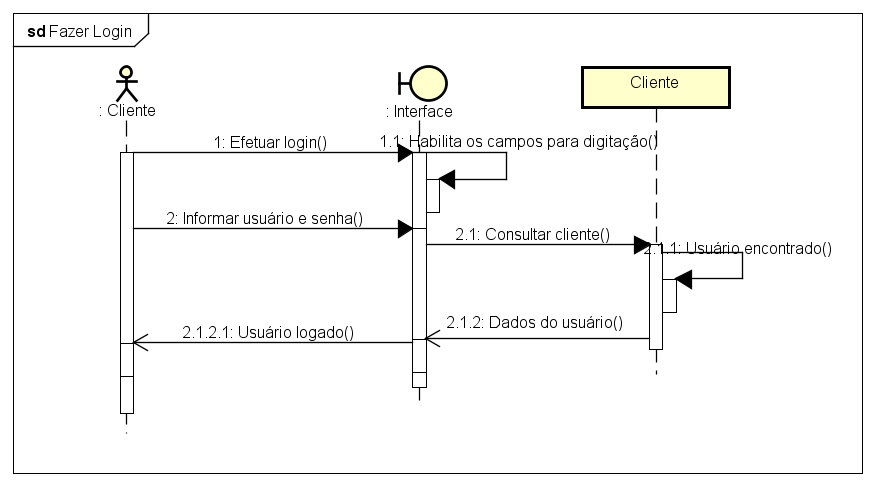
\includegraphics[width=1.0\textwidth]{./dados/figuras/7}
    \fonte{Autor}
    \label{fig:figura-6}
\end{figure}
O diagrama de sequência da Figura \ref{fig:figura-6} trata-se do passo a passo para fazer o login considerando que o usuário já foi cadastrado anteriormente.

\begin{figure}[H]
    \centering
    \caption{Diagrama de Sequência - Realizar Cadastro}
    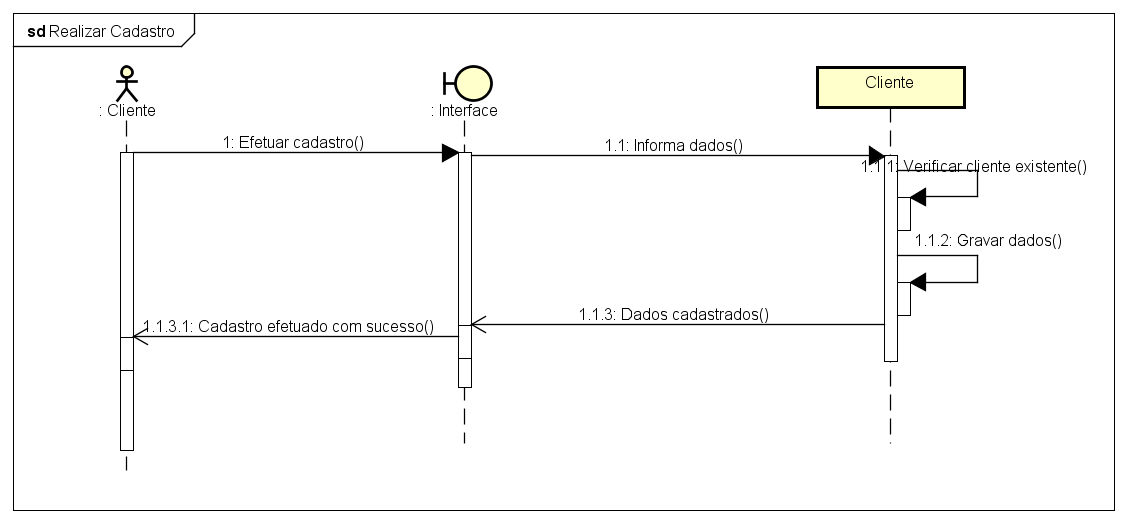
\includegraphics[width=1.0\textwidth]{./dados/figuras/8}
    \fonte{Autor}
    \label{fig:figura-7}
\end{figure}
O diagrama de sequência da Figura \ref{fig:figura-7} trata-se do passo a passo para realizar o cadastro considerando que o usuário ainda não foi cadastrado e por este motivo não encontra-se no banco de dados.

\begin{figure}[H]
    \centering
    \caption{Diagrama de Sequência - Realizar Compra}
    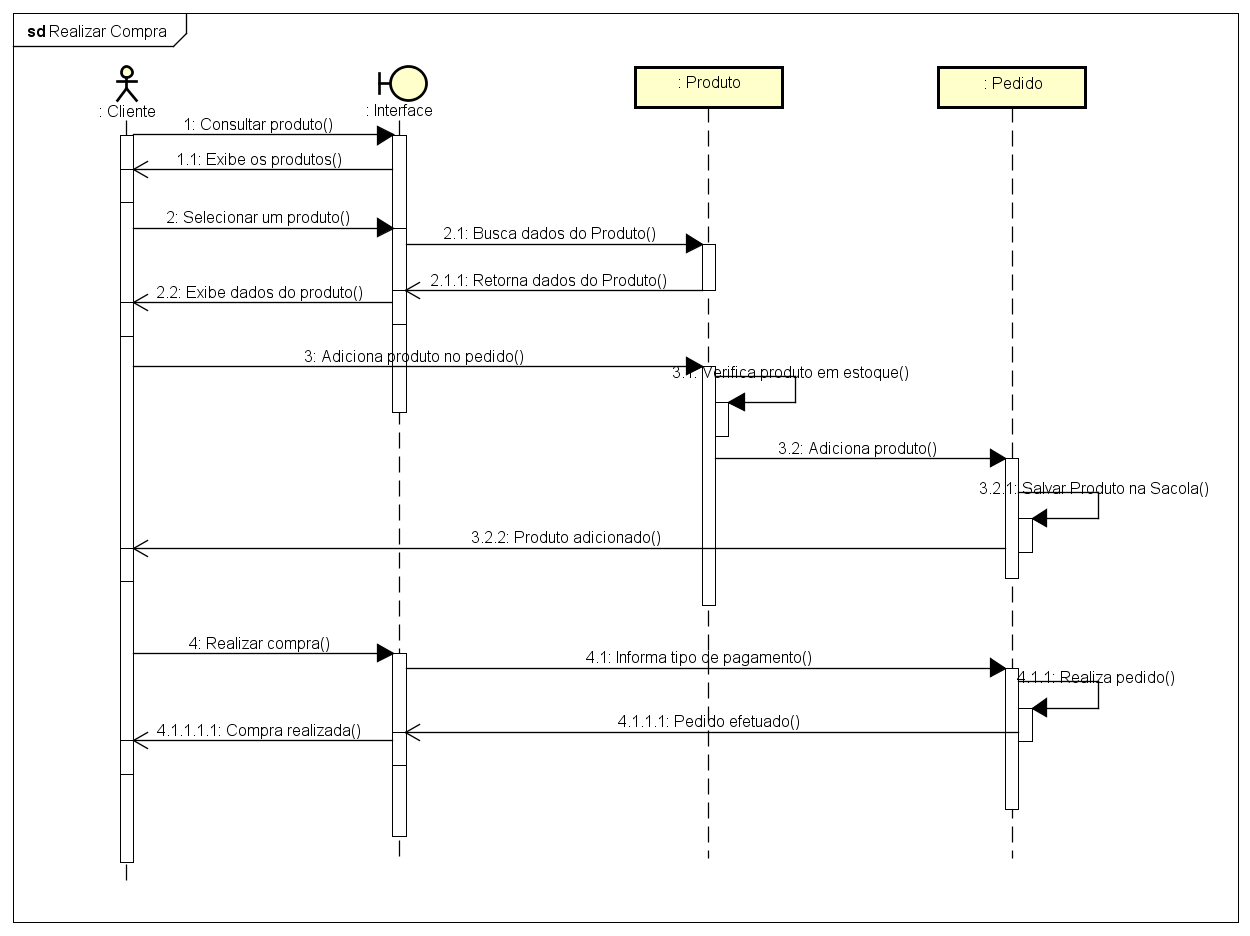
\includegraphics[width=1.0\textwidth]{./dados/figuras/9}
    \fonte{Autor}
    \label{fig:figura-8}
\end{figure}
O diagrama de sequência da Figura \ref{fig:figura-8} trata-se do passo a passo para realizar a compra dos produtos, juntamente com o processo de adicionar o produto na sacola.

%%% Diagrama de Atividade--------------
\subsection{Construção do Diagrama de Atividade}
\label{sec:diaati}
Diagrama de atividade trata-se do fluxo de operações que o trabalho seguirá. Neste diagrama é esquematizado as decisões que o site poderá ocasionar para o usuário, isso significa que em certas situações o usuário precisará realizar uma decisão, de fazer uma ou outra coisa.

\begin{figure}[H]
    \centering
    \caption{Diagrama de Atividade}
    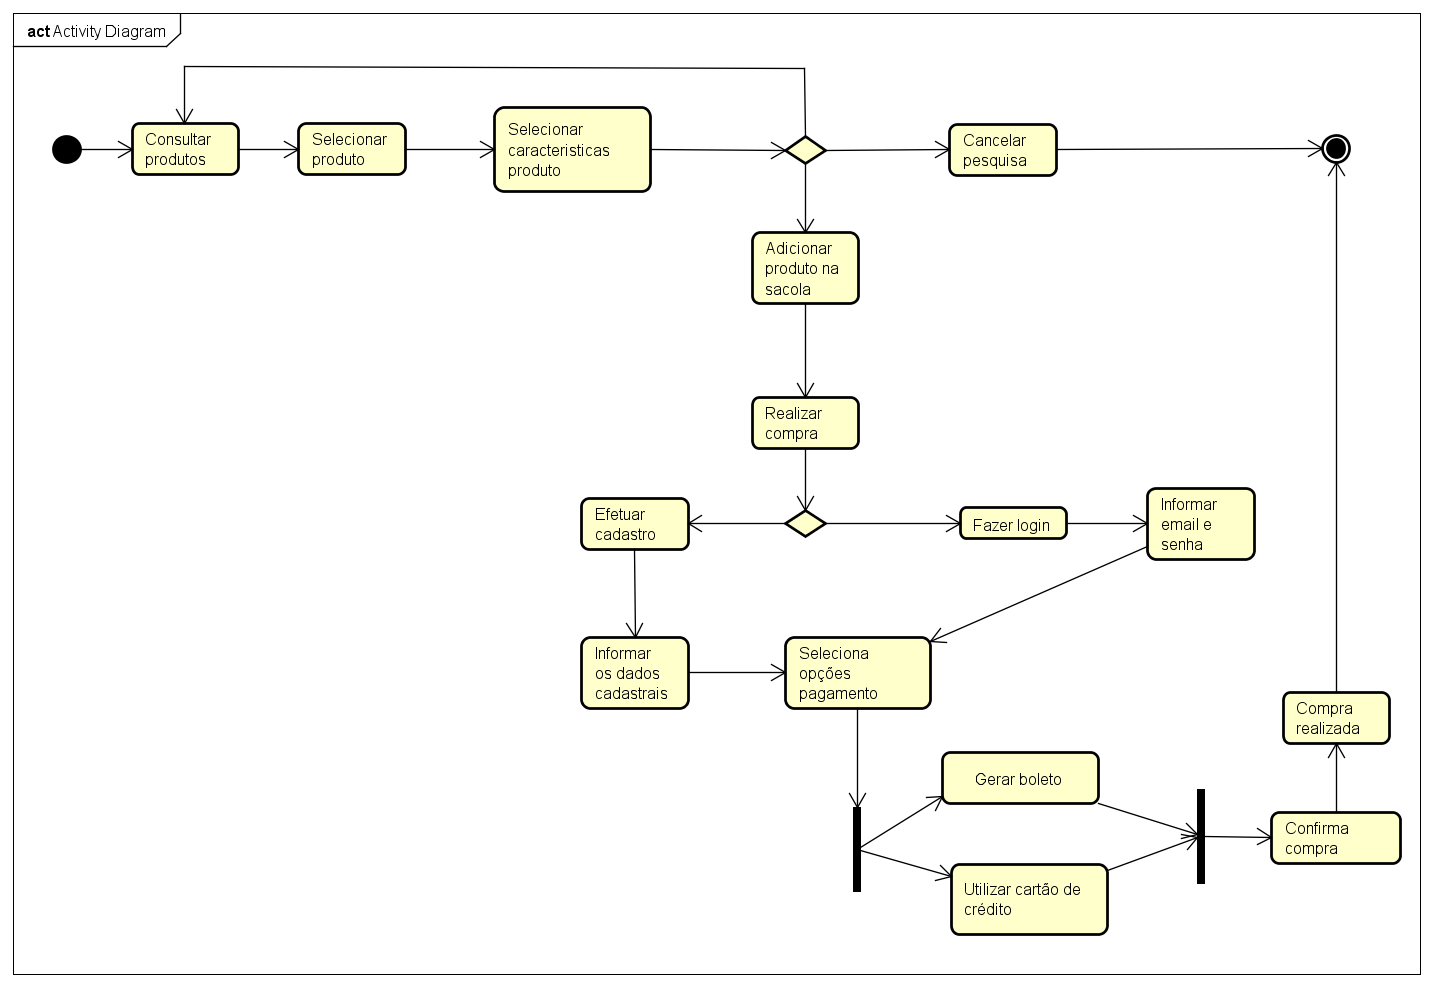
\includegraphics[width=1.0\textwidth]{./dados/figuras/6}
    \fonte{Autor}
    \label{fig:figura-9}
\end{figure}

A Figura \ref{fig:figura-9} representa o diagrama de atividade onde está sendo simulado o fluxo principal do site. 
%-----------------------------------------------------------------------------------------------------------